\documentclass[a4j]{jsarticle}

\usepackage{amsmath}
\usepackage[dvipdfmx]{graphicx}

\graphicspath{{./image/}}

\pagestyle{empty}

\title{ワイヤー一本で素粒子をとらえる}
\date{}

\begin{document}

\maketitle 

\section{目的}
宇宙線とは宇宙で生成・加速された高エネルギー荷電粒子のことを指し,そのエネルギーの高さにより素粒子の発見等の助けとなっている。宇宙線は宇宙から大気中に入射する放射線である一次宇宙線,大気の分子と反応して発生する放射線である二次宇宙線に分けられる。本実験では二次宇宙線である$\mu$粒子強度の天頂角を調べる。また,計測に用いる比例計数管の性能を確かめる予備実験として$\rm{X}$線/$\beta$線の実験も行い,それらを通して比例計数管内および$\rm{X}$線との相互作用の物理現象についても学ぶ。

\section{原理}
	\subsection{$\mu$粒子の生成}
	宇宙線の寿命は短くほとんどは地上に到達できないが,その中でも相対論効果により地上に到達することができるものの多くが$\mu$粒子である。$\mu$粒子は約$10\rm{GeV}$ほどの大きなエネルギーを持ち,そのフラックスは$1\rm{cm}^2$あたり1分間に1個程度である。これらは大気中でパイオンやケーオンのレプトンへの崩壊から次のように生成される。
	\[
	\pi^{+} \to \mu^{+} + \nu_{\mu}
	\]
	\[
	\pi^{-} \to \mu^{-} + \overline{\nu}_{\mu}
	\]
	\[
	K^{+} \to \mu^{+} + \nu_{\mu}
	\]
	\[
	K^{-} \to \mu^{-} + \overline{\nu}_{\mu}
	\]
	

	\subsection{比例計数管}
	我々は宇宙線を直接観測することはできないため,比例計数管を用いることで宇宙線の入力を信号化する。内部には$\rm{Ar}$と$\rm{CH_4}$が$9:1$の割合で混ぜられた気体P10ガスを入れた。ここでは比例計数管の構造と内部で起こる現象について説明する。\\
	\quad 透過力が高い宇宙線は比例計数管に侵入することができる。そこでガスを構成する粒子に衝突して気体粒子が電離を起こす。その電子は比例計数管内の電場により中心方向に向かって加速される。この電離電子がさらなる電子を起こす(アバランシェ増幅)。この電子が陽極である比例計数管中心を通るワイヤーを通り,ワイヤーの電圧を変化させる。つまり,宇宙線の入力を気体分子による電離電子で増幅してその電子の信号を読み取るという仕組みである。
	\begin{figure}[htbp]
	\centering
	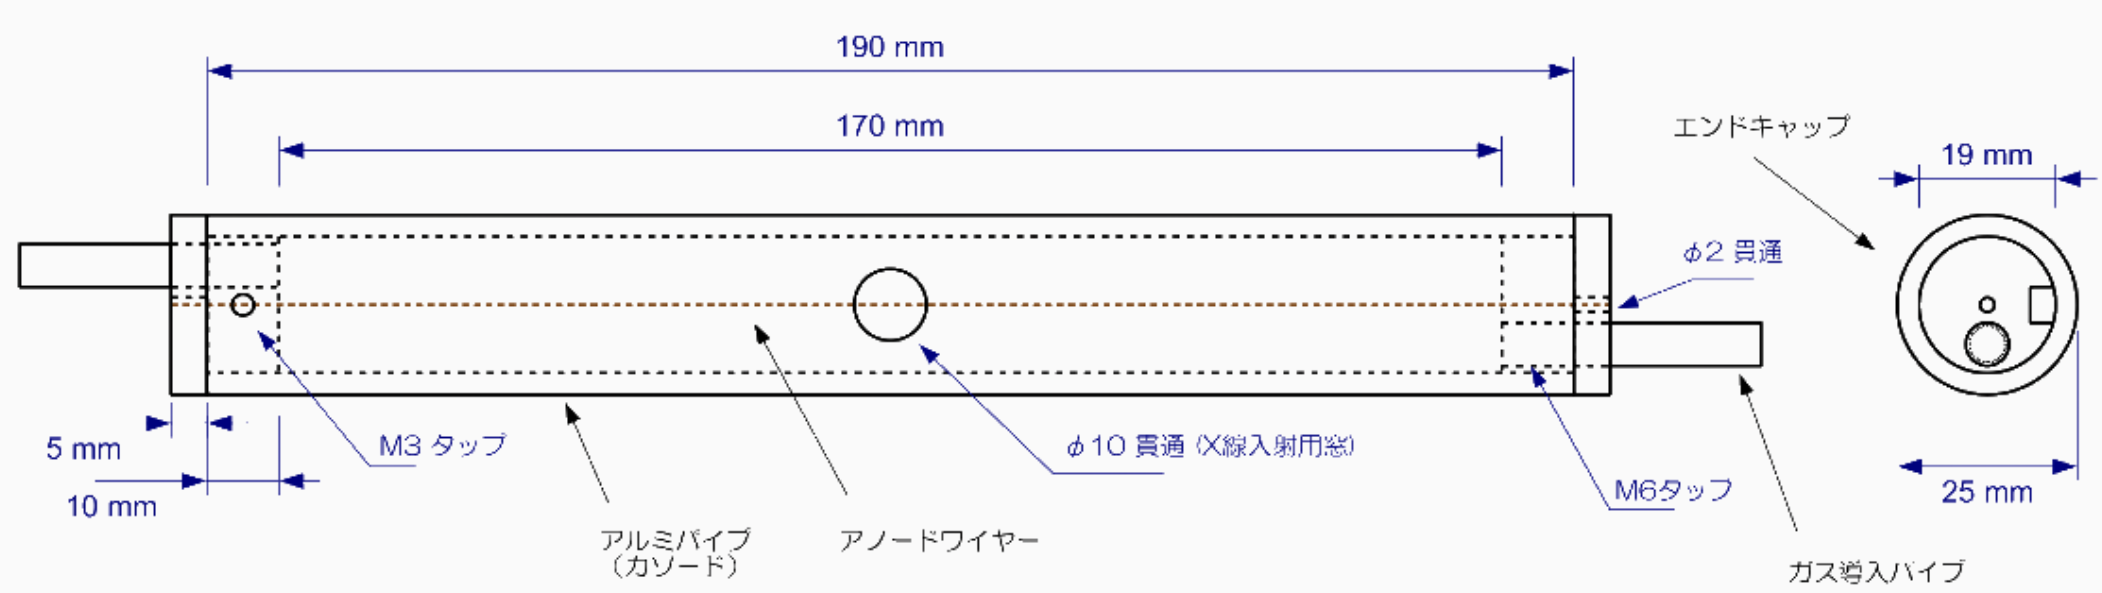
\includegraphics[width=12cm]{proportionalcounter.png}
	\caption{比例計数管の構造}
	\end{figure}
	
	\subsection{$\rm{X}$線}
	$\rm{X}$線源として$\rm{^{55}Fe}$を用いた。これは$\rm{^{55}Mn}$の基底状態へ電子捕獲反応で崩壊し,その際に$5.9\rm{keV}$の$\rm{X}$線を放出する。本実験では比例計数管へのX線の侵入に伴いArとの相互作用によりArの電子が電離する。その電離機構の一つが光電効果である。たとえば,光電効果によってK殻の電子が飛び出る。それにより空いたK殻の電子の領域に対してL殻の電子がK殻に落ちてくることで特性X線が発生する。このX線そのものは観測できないが,このX線も再び電離を引き起こす。また,M殻の電子については入射X線と束縛エネルギーの差分だけのエネルギーを持った電子が弾き飛ばされる。この電子のことをオージェ電子という。これら電離によって出た電子のエネルギーを合計すると主ピークの値になる。主に起こる反応はK殻に対しての光電効果であるため,光電効果により出た電子のエネルギーが副ピークの値になる。しかし,正確なエネルギーを求めるためにはあらゆる殻における光電効果やそれに伴って出てくる特性X線による影響も考えなければならないことに注意する必要がある。
		
	\subsection{$\mu$線}
	前述したが$\mu$粒子は宇宙からやってくる宇宙線の一つである。ここで宇宙線角度分布のモデルとして次のようなものを考える。
	\begin{itemize}
	\item 地表が平面であること
	\item 大気の厚さが一定であること
	\item 宇宙線が等方的に飛来すること
	\end{itemize}
	このモデルのもと,宇宙線強度の天頂角分布について考える。平均自由行程$\lambda$で宇宙線の強度が$1/e$になるとすれば,地表からの高さX,天頂角$\theta$における宇宙線の強度について以下の式が成り立つ。
	\begin{eqnarray}
	J(X,\theta) = J(X,\theta = 0) \frac{J(\frac{X}{\cos\theta},\theta = 0)}{J(X,\theta = 0)} \\
	J(X,\theta = 0) = J_{0} \rm{exp} \left[ -\frac{\textit{X}}{\lambda} \right]
	\end{eqnarray}
	上の2式より$\theta<<1$のときの宇宙線の強度は
	\begin{equation}
	J(X,\theta) = J_{0} \rm{exp}  \left[ -\frac{\textit{X}}{\lambda} \left( \frac{1}{\cos \theta} -1 \right) \right]  \approx \textit{J}_{0} \cos^{\alpha} \theta
	\end{equation}
	ただし,$\alpha=X/\lambda$とした。また,先行結果によると$\alpha=2$程度であることが知られている。
	
	
	\subsection{質量吸収係数}
	比例計数管の性能を確かめる予備実験としてアルミホイルの質量吸収係数を調べる実験を行った。ここでは計算方法については省略するが,注意することは厚みの単位として厚み[cm]に密度をかけた量[g/$\rm{cm^2}$]を使用する点である。これは厚み[cm]が温度の変化に伴って伸び縮みするためである。
	
	\subsection{回路}
	\begin{figure}[htbp]
	\centering
	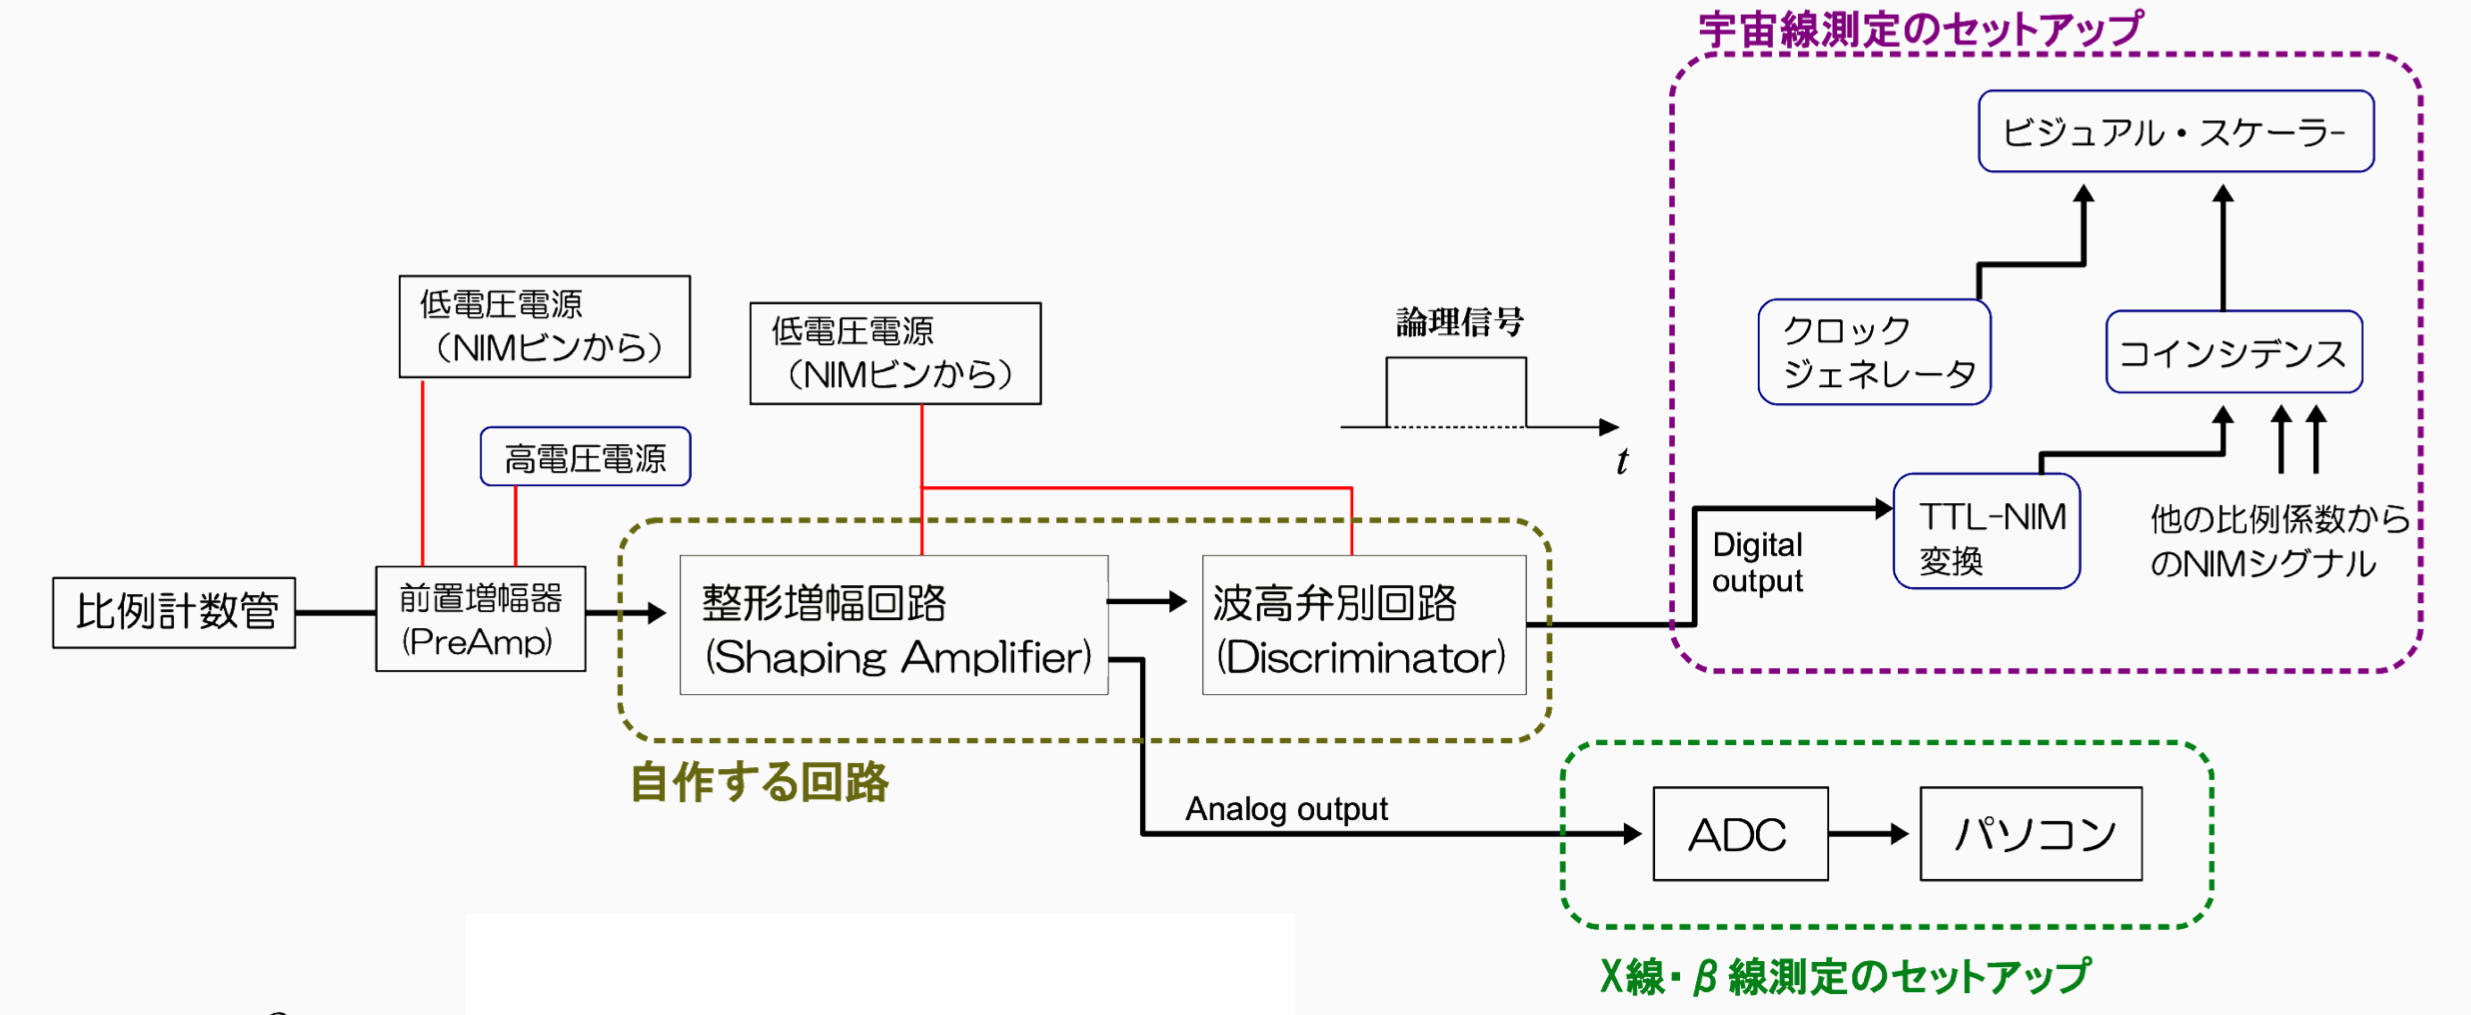
\includegraphics[width=12cm]{aboutcircuit.png}
	\caption{回路の概要}
	\end{figure}
	比例計数管により得られた電荷に対して前置増幅器により電圧に変換する。整形増幅回路はCR微分回路とRC積分回路で構成されている。CR微分回路により時間変化の小さい領域を取り除き、RC積分回路によりそれを積分することで電圧にもどすという仕組みである。波高弁別回路では整形増幅回路でできたアナログ信号を入力信号として,ある一定電圧(閾値)を超えた場合にデジタル信号を出力するというものである。X線, の実験については整形増幅回路で得られたアナログ信号をADCに通すことで各電圧のカウント数をパソコンで計測した。また,宇宙線については波高弁別回路で得られたデジタル信号,TTLシグナルをNIMシグナルに変換した。このNIMシグナルをコインシデンスに入力し,複数の比例計数管からのNIMシグナルが論理信号の出力時間で重なった場合にコインシデンスから出力がなされる。この信号が現れた回数をビジュアルスケーラーにてカウントした。
	
\section{実験手順}
	\subsection{$\rm{X}$線}
	\begin{enumerate}
	\item $\rm{^{55}Fe}$からの$\rm{X}$線を用い,高電圧$1.5\rm{kV}$をかけた状態で出力をオシロスコープで観測した。
	\item 整形増幅回路の出力をADC(MCA)に入れ,波高分布のデータを測定した。
	\item 同様の実験を$1.5\rm{kV}$から$20\rm{V}$ずつ下げて行い,高電圧が$1.42\rm{kV}$まで行った。
	\item 高電圧を$1.5\rm{kV}$にした状態で$\rm{X}$線入射窓と線源の間にアルミフォイルを一枚ずつ挟みカウント数を測定した。
	\end{enumerate}
		
	\subsection{$\mu$線}
	\begin{enumerate}
	\item 図のようにホルダーに比例計数管を複数本セットし、配線を行った。
	\item 高電圧$1.5\rm{kV}$をかけた状態でアナログ出力をオシロスコープで観測し,トリガーや整形増幅回路内の可変抵抗を操作することで信号の大きさを確認した。
	\item スケーラーを動かしカウントを行った。数時間単位などのできるだけ長い時間をとったほうが良いと思われる。大体$1$分に1個カウントするかしないかのオーダーであった。
	\item ホルダーの角度を様々に取りカウント数を測定し,宇宙線強度の天頂角分布を求めた。
	\end{enumerate}
	
\section{実験結果}
	\subsection{$\rm{X}$線}
	図\ref{x1}〜\ref{x4}がX線の実験によるデータである。図\ref{x1}において高電圧を上げることでピークのチャンネル数が大きくなっていることがわかる。図\ref{rex1}についてピークの値をエネルギーの単位で考えると5.9keVであるから,ある高電圧におけるエネルギーとピークのチャンネル数の関係がわかる。図\ref{rex2}についてピークに対する統計的ゆらぎは高電圧に関わらず一定であることがわかる。図\ref{x2}は高電圧1504Vでの各チャンネルにおける1秒当たりのカウント数を調べたものであり,右側は主ピークについてガウス関数でフィットしたものである。それぞれのデータでこのようなフィットを行い,その関数からチャンネル数などを読み取った。図\ref{x3}ではアルミフォイルの厚さに対してどれほどX線が減少するかを示したものである。図\ref{x4}は図\ref{x3}の結果によって計算できる質量吸収係数と理論値との比較である。
	
	\begin{figure}[htbp]
	\centering
	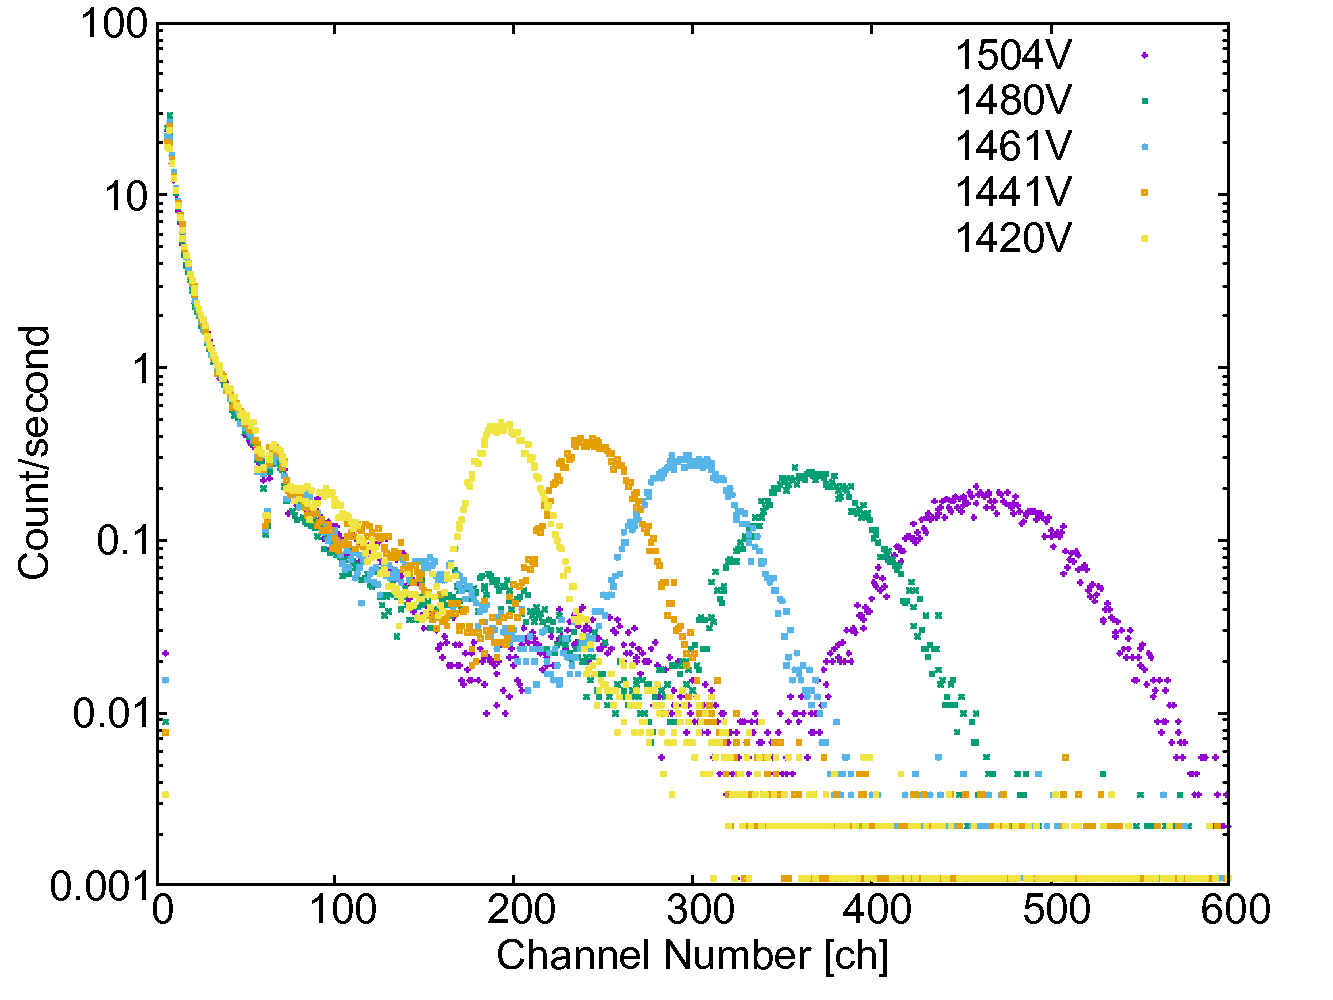
\includegraphics[width=12cm]{xray_difvoltage.pdf}
	\caption{各電圧ごとのスペクトルピーク}
	\label{x1}
	\end{figure}
	
	\begin{figure}[htbp]
	\centering
	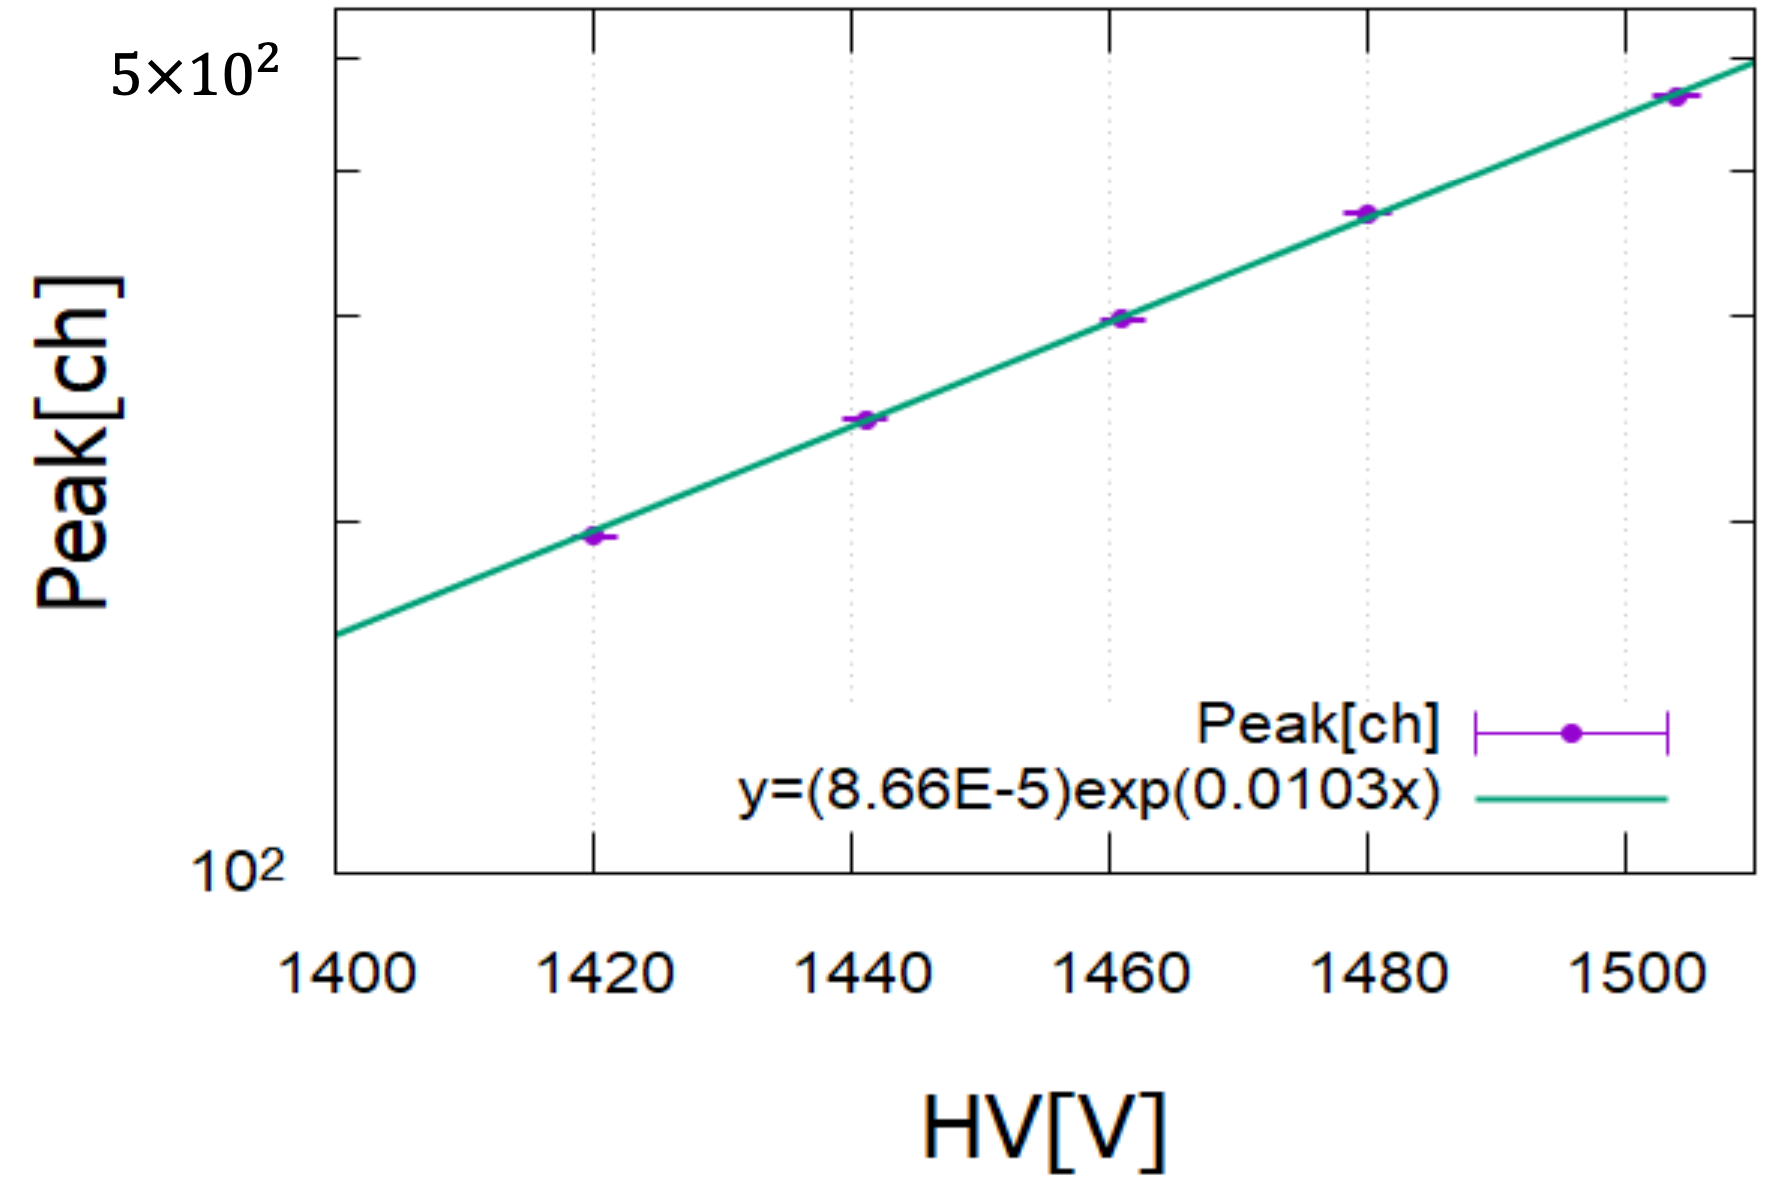
\includegraphics[width=12cm]{relation_ch+hivol.png}
	\caption{ピーク位置の高電圧依存性}
	\label{rex1}
	\end{figure}
	
	\begin{figure}[htbp]
	\centering
	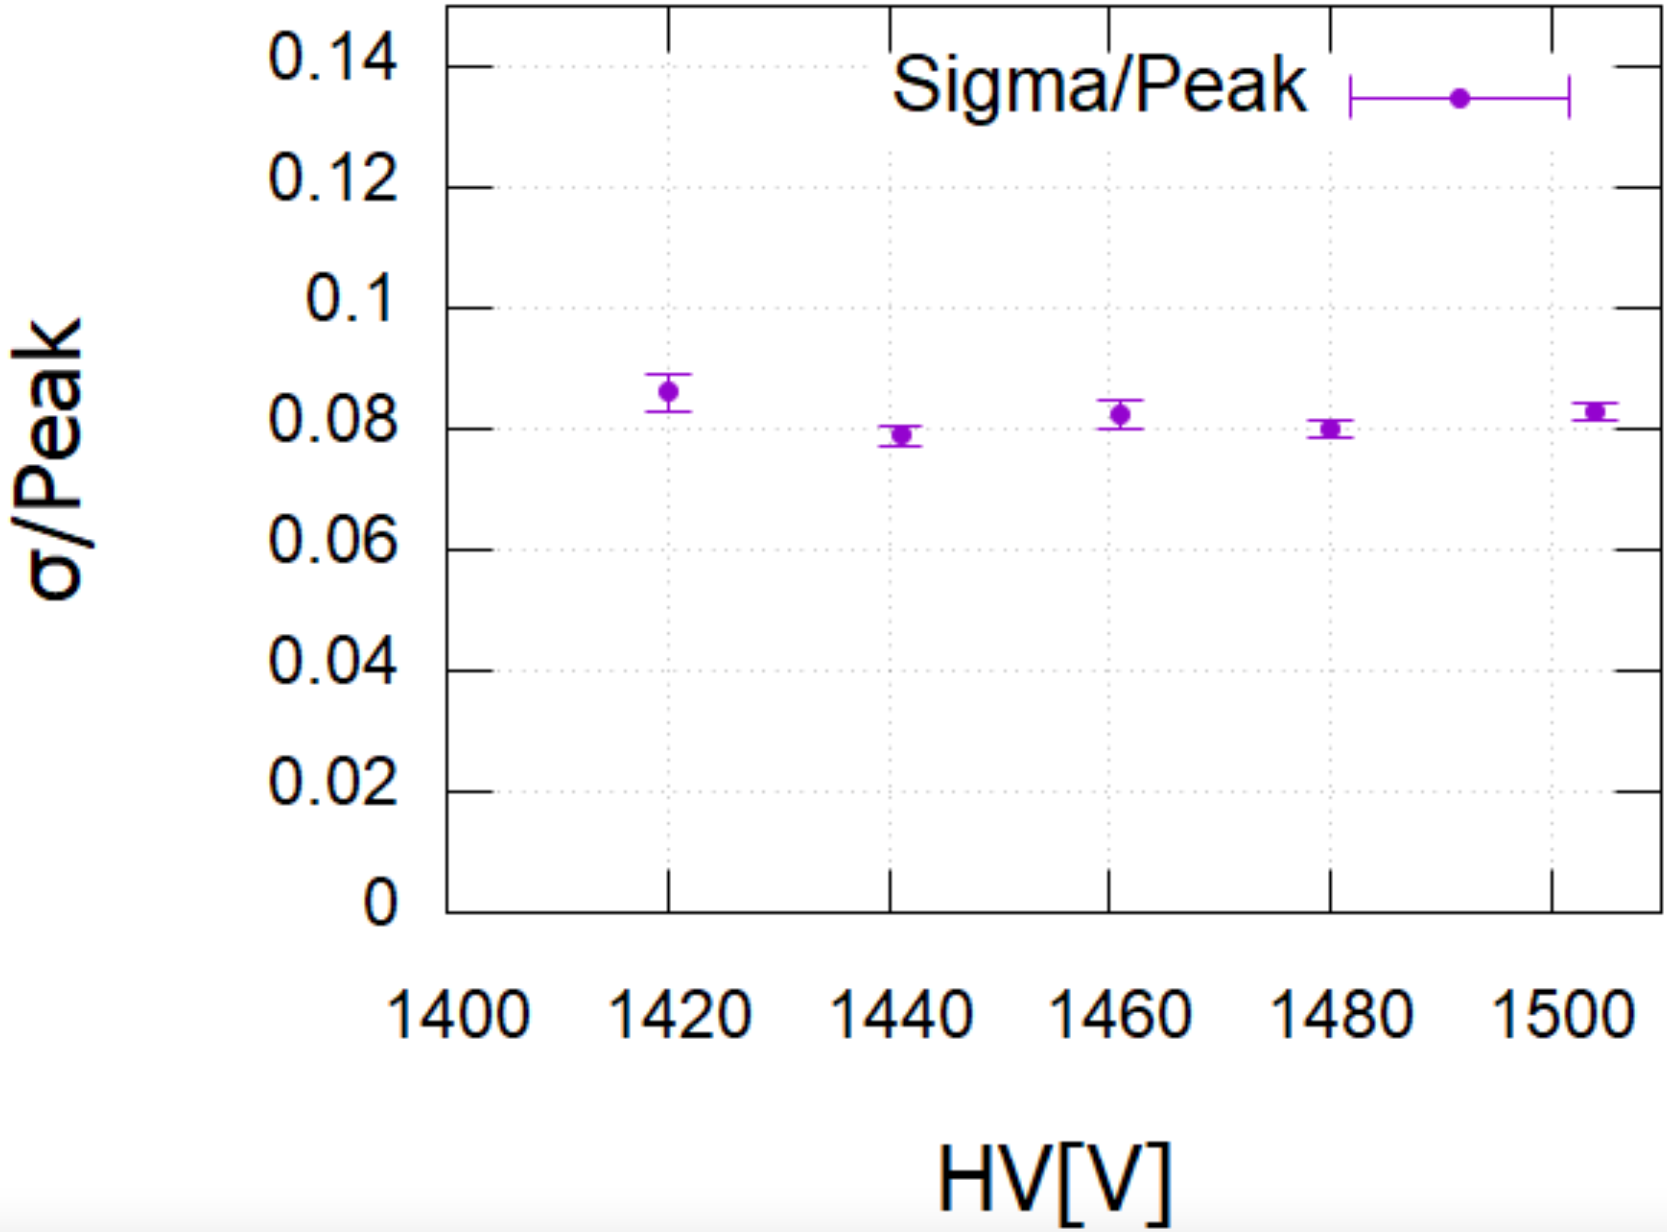
\includegraphics[width=12cm]{relation_sigmach+hivol.png}
	\caption{ピークに対する統計的ゆらぎの高電圧依存性}
	\label{rex2}
	\end{figure}
	
	\begin{figure}[htbp]
	\centering
	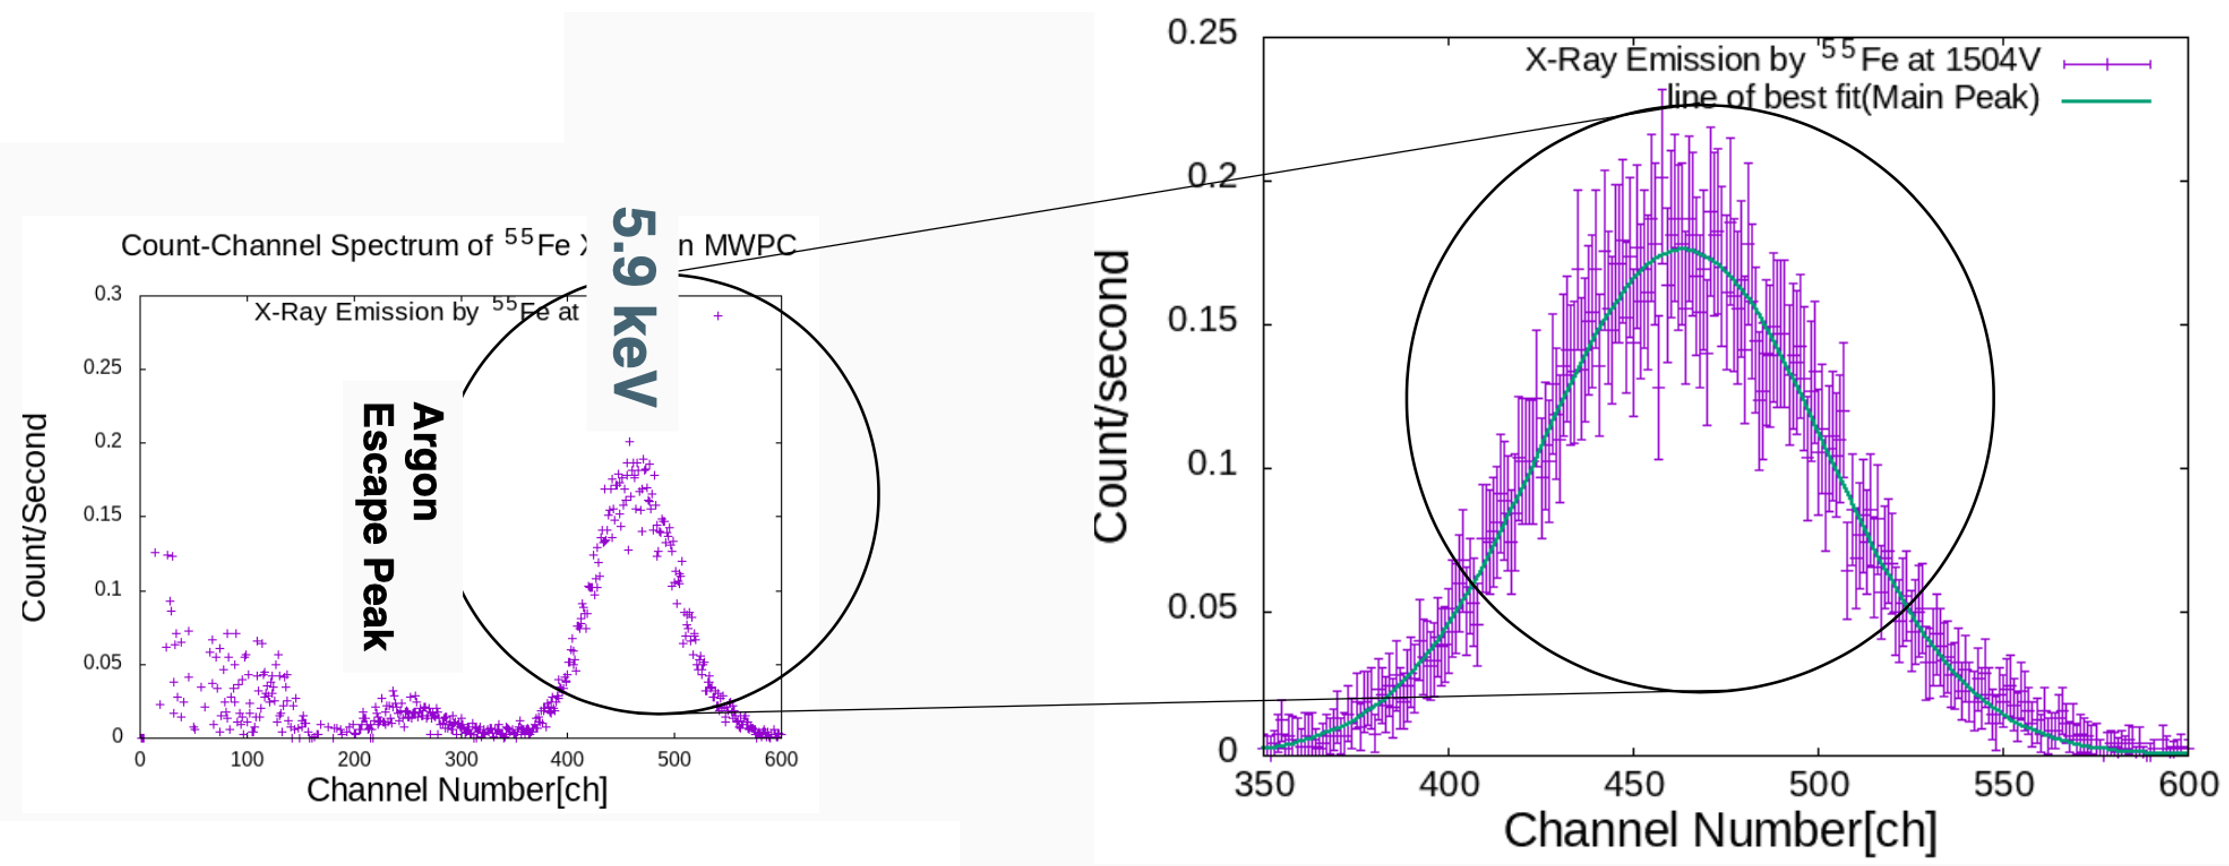
\includegraphics[width=17cm]{xray_spectrumFe55.png}
	\caption{データのフィッティング}
	\label{x2}
	\end{figure}
	
	\begin{figure}[htbp]
	\centering
	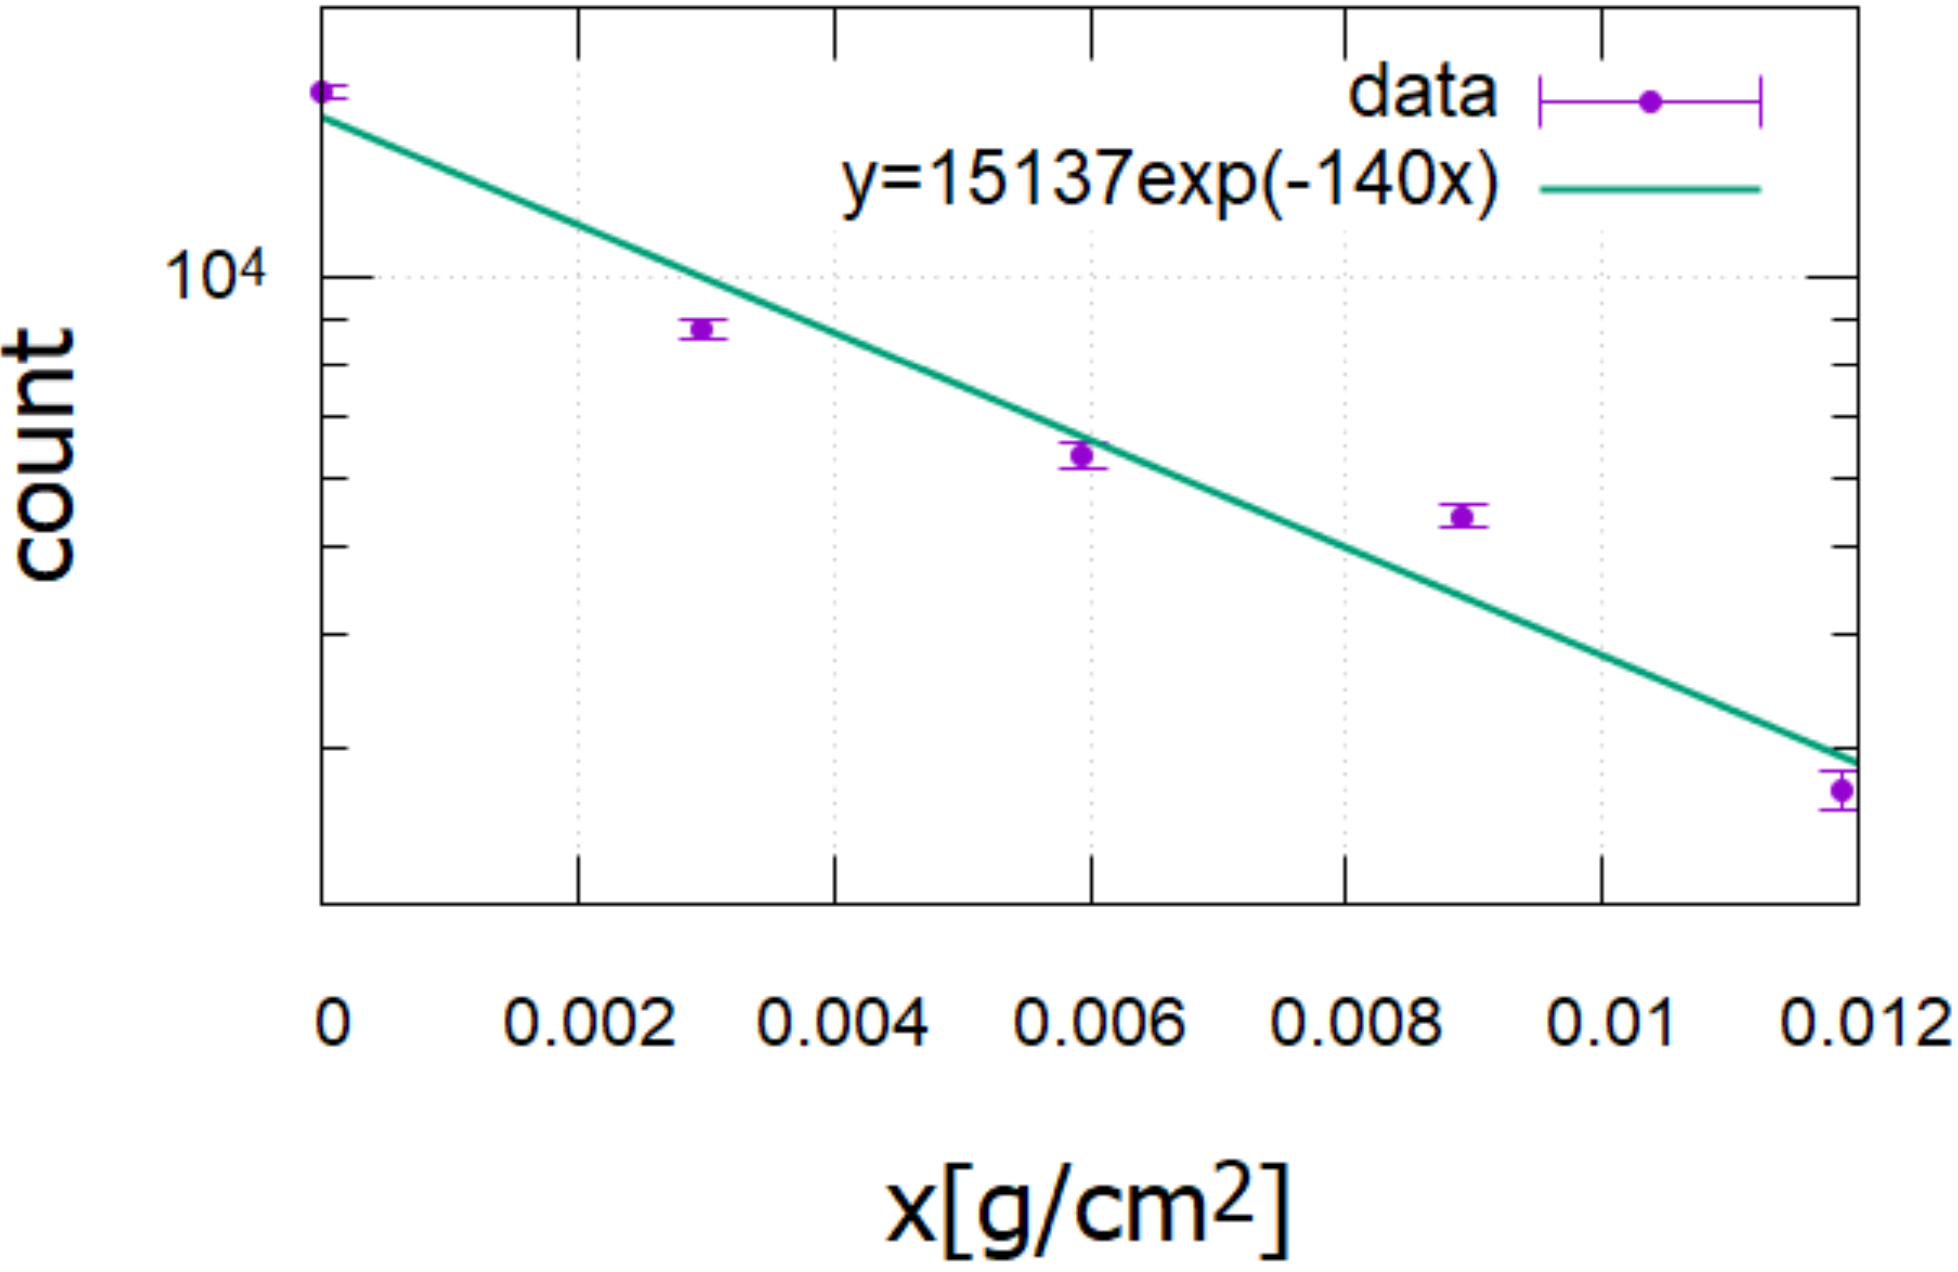
\includegraphics[width=12cm]{relation_xray+object.png}
	\caption{カウント数とアルミフォイルの厚さ}
	\label{x3}
	\end{figure}

	\begin{figure}[htbp]
	\centering
	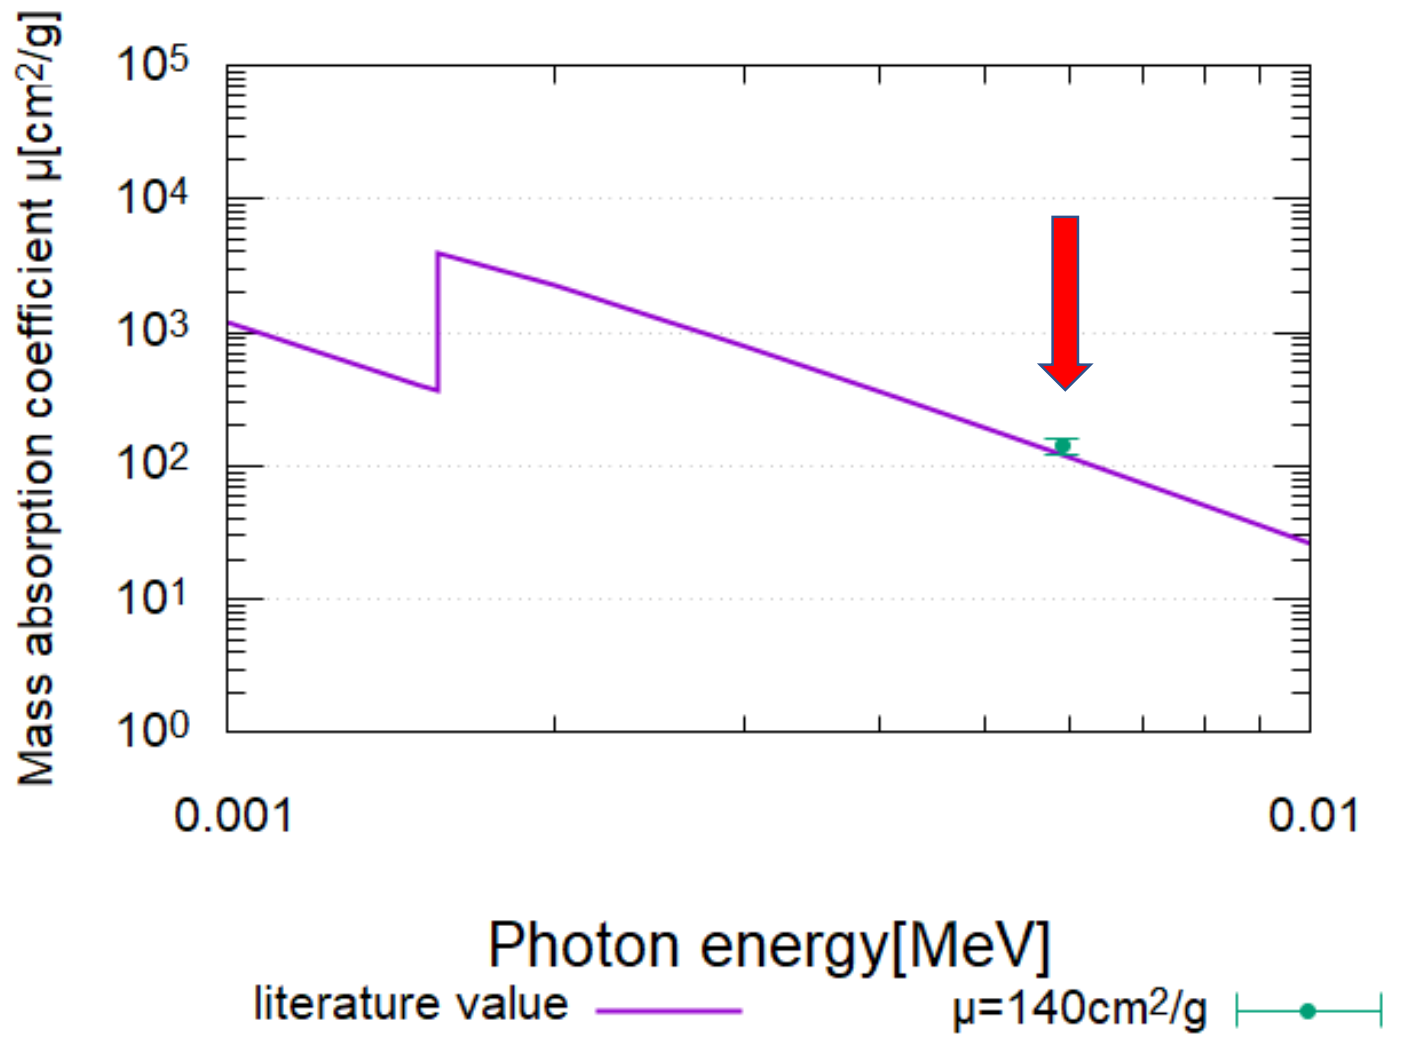
\includegraphics[width=12cm]{xray_massabs.png}
	\caption{質量吸収係数の理論値比較}
	\label{x4}
	\end{figure}
	
	\subsection{$\beta$線}
	$\beta$線については計測及び解析が間に合わなかったのでここでは省略する。
	
	\subsection{$\mu$線}
	図\ref{mu1}はミューオン強度の天頂角分布を示したものであり,大きい天頂角においては観測されるミューオンの数が少なくなっていることがわかる。また,角度に依存しないバックグラウンド定数を$C$として$\cos^{\alpha} \theta$でフィットをした。\\
	そのフィット関数$J(\theta)$ は
	\begin{gather}
	J(\theta) = J(0)\cos^{\alpha} \theta + C\\
	J(0) = 0.044 \pm 0.008 , \alpha = 4.9 \pm 2.6 , C = 0.133 \pm 0.005
	\end{gather}
	また,換算$\chi^2$値は0.52であった。
	\begin{figure}[htbp]
	\centering
	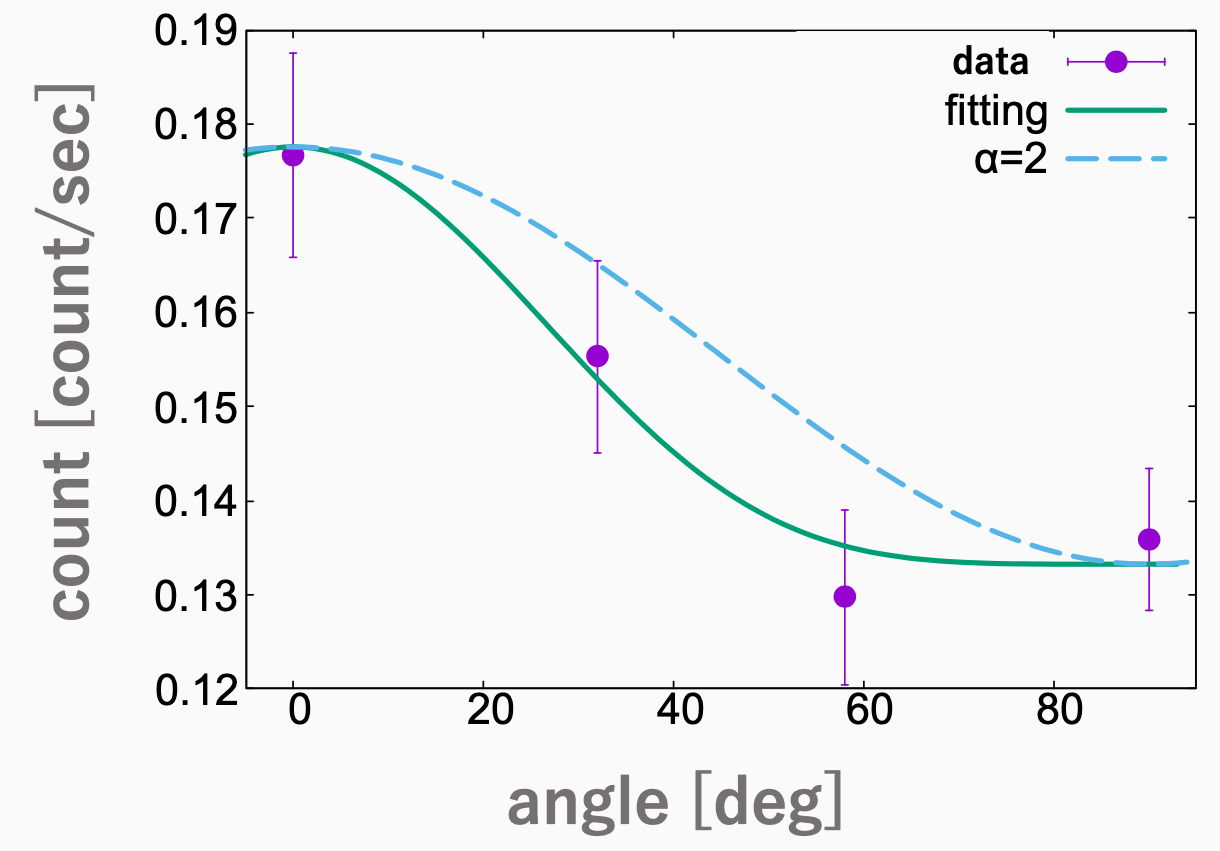
\includegraphics[width=12cm]{muon_distribution.png}
	\caption{ミューオン強度の天頂角分布}
	\label{mu1}
	\end{figure}
	
\section{考察}
$\mu$線の測定において先行研究によると$\alpha = 2$であることから,結果が$1\sigma$の範囲で先行研究より大きいことが言える。これは$90^{\circ}$でカウント数が最小になると予想されるのに対し計測では$60^{\circ}$付近で最小になっているために$\alpha$の値が大きくなってしまったと考えられる。この原因として換算$\chi^2$値が1より小さいことから,不確かさが大きいことが挙げられる。この背景として計測時にカウントレートの増減が時々見られたこと,他グループが数日単位の計測であったことに比べて計測時間が数十分と短かったことがある。改善としては,数日単位で計測を行うことが挙げられる。

\section{まとめ}
比例計数管や整形増幅器,波高弁別器を作成し,それを用いて$\mu$線強度の天頂角分布を測定したところ$\cos\theta$の$4.9 \pm 2.6$乗に比例することが実験からわかった。また, X線の予備実験を通して比例計数管原理や放射線と物質の相互作用についても学ぶことができた。

\begin{thebibliography}{99}
\bibitem{yasashi} 山崎耕造, トコトンやさしい宇宙線と素粒子の本, 2018
\bibitem{gru} C.グルーペン, 宇宙素粒子物理学, 2009
\bibitem{samatyare} 2022年度サマーチャレンジ編集委員会, サマーチャレンジ2022講義テキスト, 2022
\bibitem{tohoku} 金田雅司, ワイヤー一本で素粒子をとらえるー素粒子・原子核実験の心臓部分「ワイヤーチェンバー」を作ろうー, 2018
\end{thebibliography}

\end{document}

